\documentclass[]{article}
\usepackage{graphicx}
\usepackage{amsmath}
\usepackage{amssymb}
\usepackage{geometry}
\geometry{
	a4paper,
	left=10mm,
	top=20mm,
	right=10mm,
	left=20mm,
}

\setlength{\parindent}{0pt}

\begin{document}

\section{Current-type control with time restrictions for down $\rightarrow$ up}

\subsection{$L_1$ constraints}

\subsubsection{E population precision measurement}

\textbf{Point a}, $w_P = w_1 = 1$

\includegraphics[width=\textwidth]{../../current/gui/data_2/1_e/1_e_20.jpg}

\begin{itemize}
	\item discontinuities for small $T$
	\item $u_E$ is faster 
\end{itemize}
\newpage

\textbf{Point a}, $w_P = 1, w_1 = \text{max}$

\includegraphics[width=\textwidth]{../../current/gui/data_2/1_e/1_e_20_Wmax.jpg}
\newpage

\textbf{Point b}, $w_P = w_1 = 1$

\includegraphics[width=\textwidth]{../../current/gui/data_2/1_e/1_e_50.jpg}
\newpage

\textbf{Point b}, $w_P = 1, w_1 = \text{max}$

\includegraphics[width=\textwidth]{../../current/gui/data_2/1_e/1_e_50_Wmax.jpg}
\newpage

%%%%%%%%%%%%%%%%%%%%%%%%%%%%%%%%%%%%%%%%%%%%%%%%%%%%%%
\subsubsection{I population precision measurement}

\textbf{Point a}, $w_P = w_1 = 1$

\includegraphics[width=\textwidth]{../../current/gui/data_2/1_i/1_i_20.jpg}

\begin{itemize}
	\item $r_I$ can be controlled without affecting $r_E$, presumably not vice-versa
	\item for small $T$, temporarily switching produces smaller cost
\end{itemize}

\newpage

\textbf{Point a}, $w_P = 1, w_1 = \text{max}$

\includegraphics[width=\textwidth]{../../current/gui/data_2/1_i/1_i_20_Wmax.jpg}
\newpage

\textbf{Point b}, $w_P = w_1 = 1$

\includegraphics[width=\textwidth]{../../current/gui/data_2/1_i/1_i_50.jpg}
\newpage

\textbf{Point b}, $w_P = 1, w_1 = \text{max}$


\includegraphics[width=\textwidth]{../../current/gui/data_2/1_i/1_i_50_Wmax.jpg}
\newpage

%%%%%%%%%%%%%%%%%%%%%%%%%%%%%%%%%%%%%%%%%%%%%%%%%%%%%%
\subsubsection{EI population precision measurement}

\textbf{Point a}, $w_P = w_1 = 1$

\includegraphics[width=\textwidth]{../../current/gui/data_2/1_ei/1_ei_20.jpg}
\newpage

\textbf{Point a}, $w_P = 1, w_1 = \text{max}$

\includegraphics[width=\textwidth]{../../current/gui/data_2/1_ei/1_ei_20_Wmax.jpg}
\newpage

\textbf{Point b}, $w_P = w_1 = 1$

\includegraphics[width=\textwidth]{../../current/gui/data_2/1_ei/1_ei_50.jpg}
\newpage

\textbf{Point b}, $w_P = 1, w_1 = \text{max}$

\includegraphics[width=\textwidth]{../../current/gui/data_2/1_ei/1_ei_50_Wmax.jpg}
\newpage

\subsection{$L_2$ constraints}

\subsubsection{E population precision measurement}

\textbf{Point a}, $w_P = w_1 = 1$

\includegraphics[width=\textwidth]{../../current/gui/data_2/2_e/2_e_20.jpg}
\newpage

\textbf{Point a}, $w_P = 1, w_1 = \text{max}$

\includegraphics[width=\textwidth]{../../current/gui/data_2/2_e/2_e_20_Wmax.jpg}
\newpage

\textbf{Point b}, $w_P = w_1 = 1$

\includegraphics[width=\textwidth]{../../current/gui/data_2/2_e/2_e_50.jpg}
\newpage

\textbf{Point b}, $w_P = 1, w_1 = \text{max}$

\includegraphics[width=\textwidth]{../../current/gui/data_2/2_e/2_e_50_Wmax.jpg}
\newpage

%%%%%%%%%%%%%%%%%%%%%%%%%%%%%%%%%%%%%%%%%%%%%%%%%%%%%%
\subsubsection{I population precision measurement}

\textbf{Point a}, $w_P = w_1 = 1$

\includegraphics[width=\textwidth]{../../current/gui/data_2/2_i/2_i_20.jpg}
\newpage

\textbf{Point a}, $w_P = 1, w_1 = \text{max}$

\includegraphics[width=\textwidth]{../../current/gui/data_2/2_i/2_i_20_Wmax.jpg}
\newpage

\textbf{Point b}, $w_P = w_1 = 1$

\includegraphics[width=\textwidth]{../../current/gui/data_2/2_i/2_i_50.jpg}
\newpage

\textbf{Point b}, $w_P = 1, w_1 = \text{max}$

\includegraphics[width=\textwidth]{../../current/gui/data_2/2_i/2_i_50_Wmax.jpg}
\newpage

%%%%%%%%%%%%%%%%%%%%%%%%%%%%%%%%%%%%%%%%%%%%%%%%%%%%%%
\subsubsection{EI population precision measurement}

\textbf{Point a}, $w_P = w_1 = 1$

\includegraphics[width=\textwidth]{../../current/gui/data_2/2_ei/2_ei_20.jpg}
\newpage

\textbf{Point a}, $w_P = 1, w_1 = \text{max}$

\includegraphics[width=\textwidth]{../../current/gui/data_2/2_ei/2_ei_20_Wmax.jpg}
\newpage

\textbf{Point b}, $w_P = w_1 = 1$

\includegraphics[width=\textwidth]{../../current/gui/data_2/2_ei/2_ei_50.jpg}
\newpage

\textbf{Point b}, $w_P = 1, w_1 = \text{max}$

\includegraphics[width=\textwidth]{../../current/gui/data_2/2_ei/2_ei_50_Wmax.jpg}
\newpage

\section{Rate-type control}
\bigskip

External rate:

\begin{footnotesize}
\begin{align}
	r_{\alpha \beta} (t) = \frac{c_{\alpha \beta}}{|J_{\alpha \beta}|} K_\beta \tau_{s, \beta} \cdot r_\beta (t-d_\alpha) \hspace{5mm} \rightarrow \hspace{5mm} \frac{c_{\alpha \beta}}{|J_{\alpha \beta}|} K_\beta \tau_{s, \beta} \cdot r_\beta (t-d_\alpha) + \frac{c_\text{gl}}{|J_{\alpha \beta}|} K_{\beta, \text{gl}} \tau_{s,\beta} \cdot u_{\alpha\beta}(t) \\
	\rho_{\alpha \beta} (t) = \frac{c_{\alpha \beta}^2}{J_{\alpha \beta}^2} K_\beta \tau_{s,\beta}^2 \cdot r_\beta (t-d_\alpha) \hspace{5mm} \rightarrow \hspace{5mm} \frac{c_{\alpha \beta}^2}{J_{\alpha \beta}^2} K_\beta \tau_{s,\beta}^2 \cdot r_\beta (t-d_\alpha) + \frac{c_\text{gl}^2}{J_{\alpha \beta}^2} K_{\beta, \text{gl}} \tau_{s,\beta}^2 \cdot u_{\alpha\beta}(t) \\
	\hline
	\sigma_E(t) - (\frac{2 J_{EE}^2 \sigma_{s,EE}^2(t) \tau_{s,E} \tau_m}{(1+ r_{EE} (t) ) \tau_m + \tau_{s,E}} + \frac{2 J_{EI}^2 \sigma_{s,EI}^2(t) \tau_{s,I} \tau_m}{(1+r_{EI} (t)) \tau_m + \tau_{s,I}} + {(\sigma_E^\text{ext})}^2)^{\frac{1}{2}} =0 \\
	\sigma_I(t) - (\frac{2 J_{IE}^2 \sigma_{s,IE}^2(t) \tau_{s,E} \tau_m}{(1+r_{IE}(t)) \tau_m + \tau_{s,E}} + \frac{2 J_{II}^2 \sigma_{s,II}^2(t) \tau_{s,I} \tau_m}{(1+r_{II}(t)) \tau_m + \tau_{s,I}} + {(\sigma_I^\text{ext})}^2)^{\frac{1}{2}} =0 \\
	\hline
	\dot{\overline{s}}_{EE} + \frac{\overline{s}_{EE}(t)}{\tau_{s,E}} - (1 - \overline{s}_{EE}(t)) \cdot \frac{r_{EE}(t)}{\tau_{s,E}} =0 \\
	\dot{\overline{s}}_{EI} + \frac{\overline{s}_{EI}(t)}{\tau_{s,I}} - (1 - \overline{s}_{EI}(t)) \cdot \frac{r_{EI}(t)}{\tau_{s,I}} =0 \\
	\dot{\overline{s}}_{IE} + \frac{\overline{s}_{IE}(t)}{\tau_{s,E}} - (1 - \overline{s}_{IE}(t)) \cdot \frac{r_{IE}(t)}{\tau_{s,E}} =0 \\
	\dot{\overline{s}}_{II} + \frac{\overline{s}_{II}(t)}{\tau_{s,I}} - (1 - \overline{s}_{II}(t)) \cdot \frac{r_{II}(t)}{\tau_{s,I}} =0 \\
	\hline
	\dot{\sigma}_{s,EE}^2 - \frac{1}{\tau_{s, e}^2} \left( (1 - \overline{s}_{EE}(t))^2 \cdot \rho_{EE} (t) + (\rho_{EE} (t) - 2 \tau_{s, e} (r_{EE} (t) + 1))\cdot \sigma_{s,EE}^2(t) \right)  =0 \\
	\dot{\sigma}_{s,EI}^2- \frac{1}{\tau_{s, i}^2} \left( (1 - \overline{s}_{EI}(t))^2 \cdot \rho_{EI} (t) + (\rho_{EI} (t) - 2 \tau_{s,I} (r_{EI} (t) + 1))\cdot \sigma_{s,EI}^2(t) \right) =0 \\
	\dot{\sigma}_{s,IE}^2 - \frac{1}{\tau_{s,E}^2} \left( (1 - \overline{s}_{IE}(t))^2 \cdot \rho_{IE} (t) + (\rho_{IE} (t) - 2 \tau_{s, e} (r_{IE} (t) + 1))\cdot \sigma_{s,IE}^2(t) \right) =0 \\
	\dot{\sigma}_{s,II}^2 - \frac{1}{\tau_{s,I}^2} \left( (1 - \overline{s}_{II}(t))^2 \cdot \rho_{II} (t) + (\rho_{II} (t) - 2 \tau_{s,I} (r_{II} (t) + 1))\cdot \sigma_{s, ii}^2(t) \right) =0 \\
\end{align}
\end{footnotesize}

\subsection{Down $\rightarrow$ up, $L_1$ cost}

\begin{minipage}{0.65\textwidth}
	\begin{itemize}
		\item excitatory input to excitatory population throughout bistable regime
		\item amplitude roughly proportional to horizontal distance to target regime\\
		correlation coefficient = 0.97100708
		\item total cost roughly proportional to horizontal distance to target regime\\
		correlation coefficient = 0.97867371
		\item width roughly proportional to external input to inhibitory population\\
		correlation coefficient = 0.80623448
	\end{itemize}
\end{minipage}
\begin{minipage}{0.33\textwidth}
	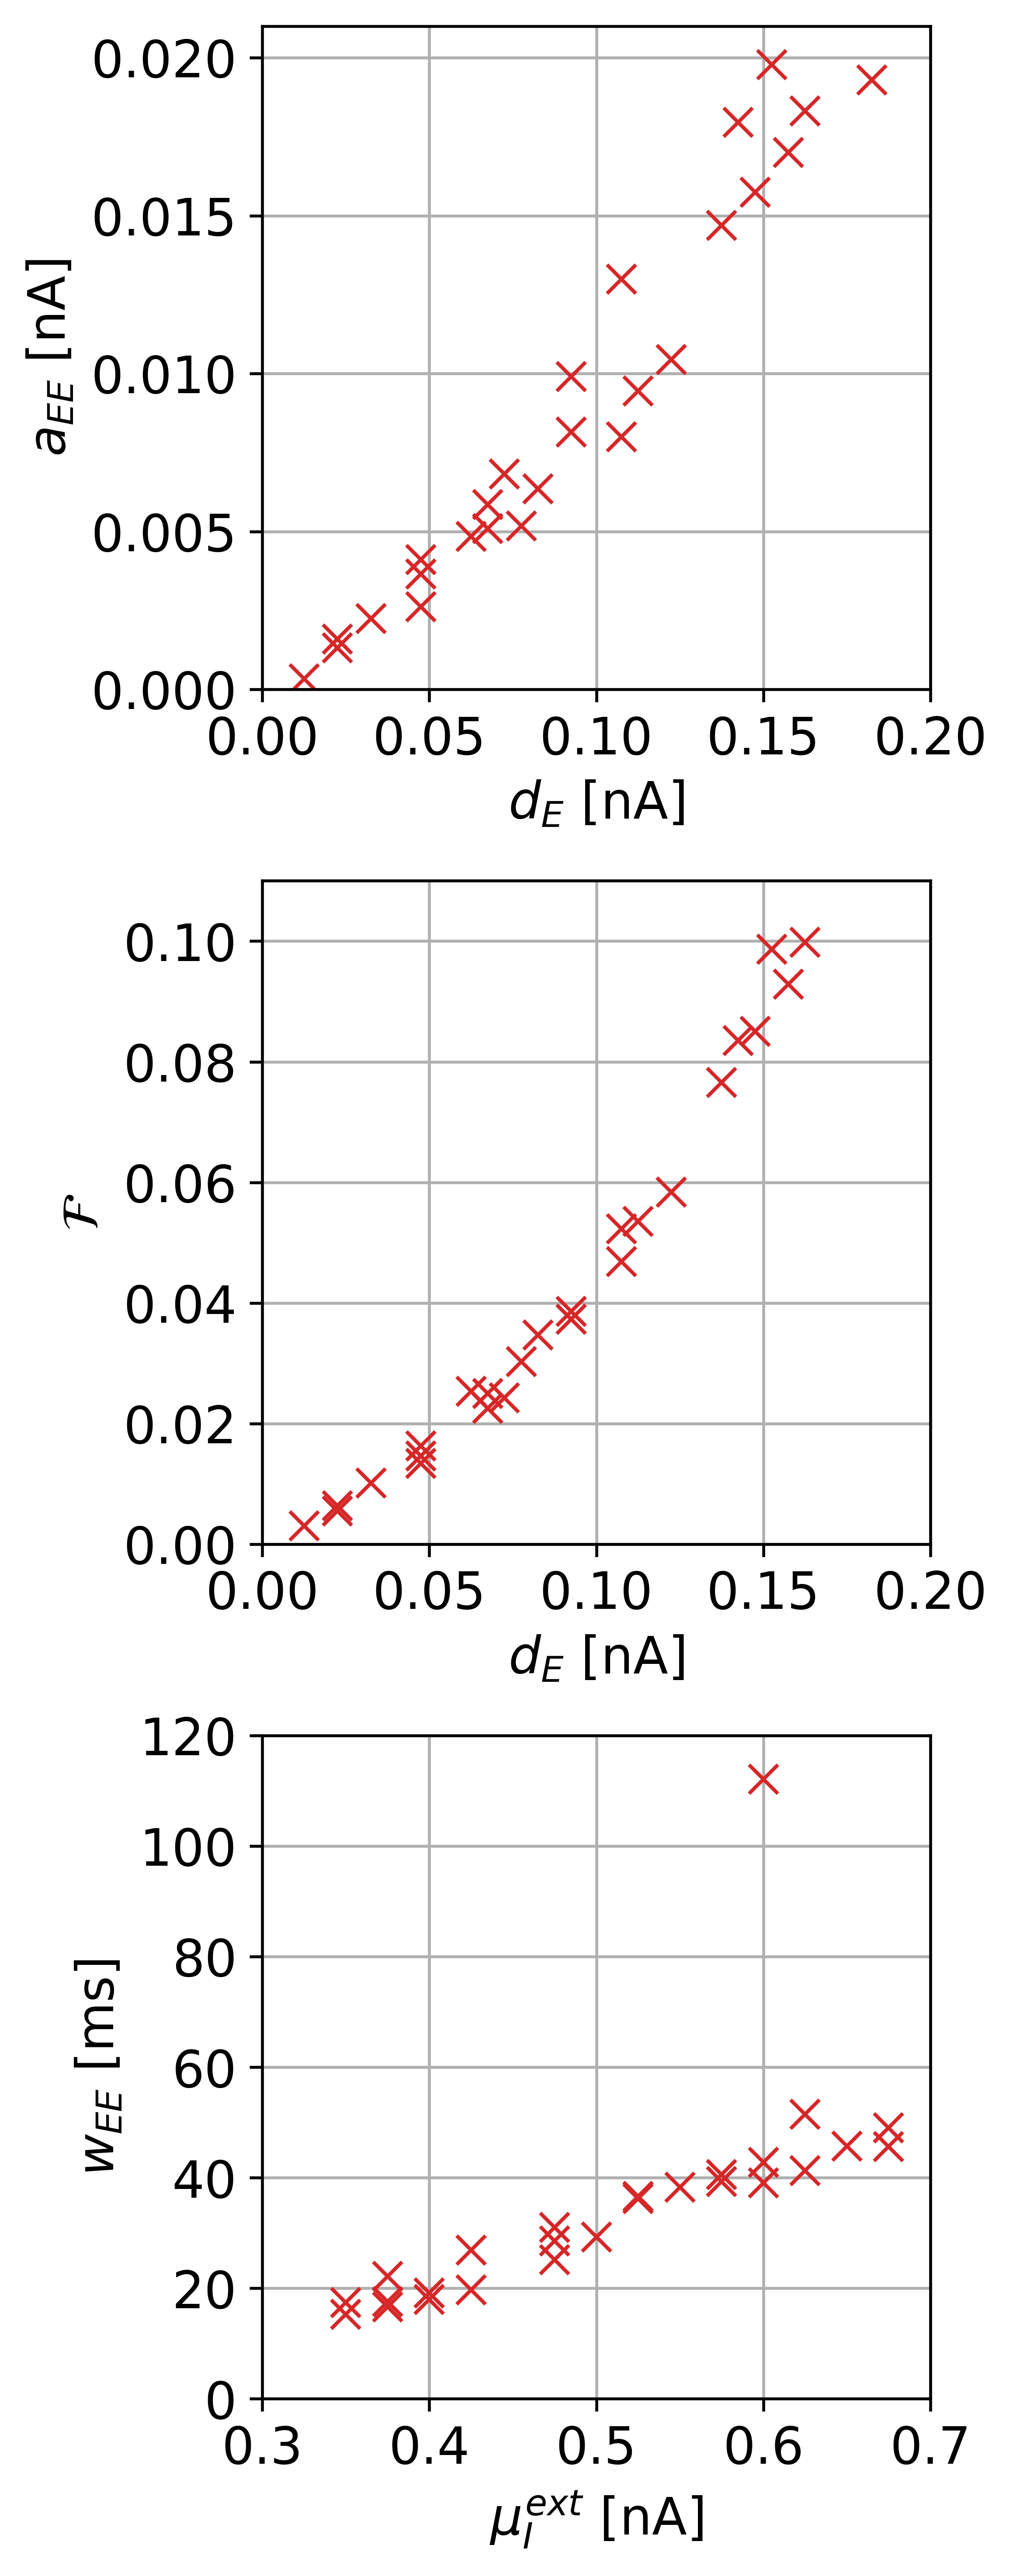
\includegraphics[width=\textwidth]{../rate_1.png}
\end{minipage}

\subsection{Down $\rightarrow$ up, $L_2$ cost}

\begin{minipage}{0.65\textwidth}
	\begin{itemize}
		\item excitatory input to excitatory population with significantly larger (factor 10) amplitude throughout bistable regime
		\item amplitude roughly proportional to horizontal distance to target regime\\
		correlation coefficient = 0.87713965
		\item total cost scales super-linearly with horizontal distance to target regime\\
		correlation coefficient = 0.35968405
		\item width roughly proportional to external input to inhibitory population\\
		correlation coefficient = 0.6869857
	\end{itemize}
\end{minipage}
\begin{minipage}{0.33\textwidth}
	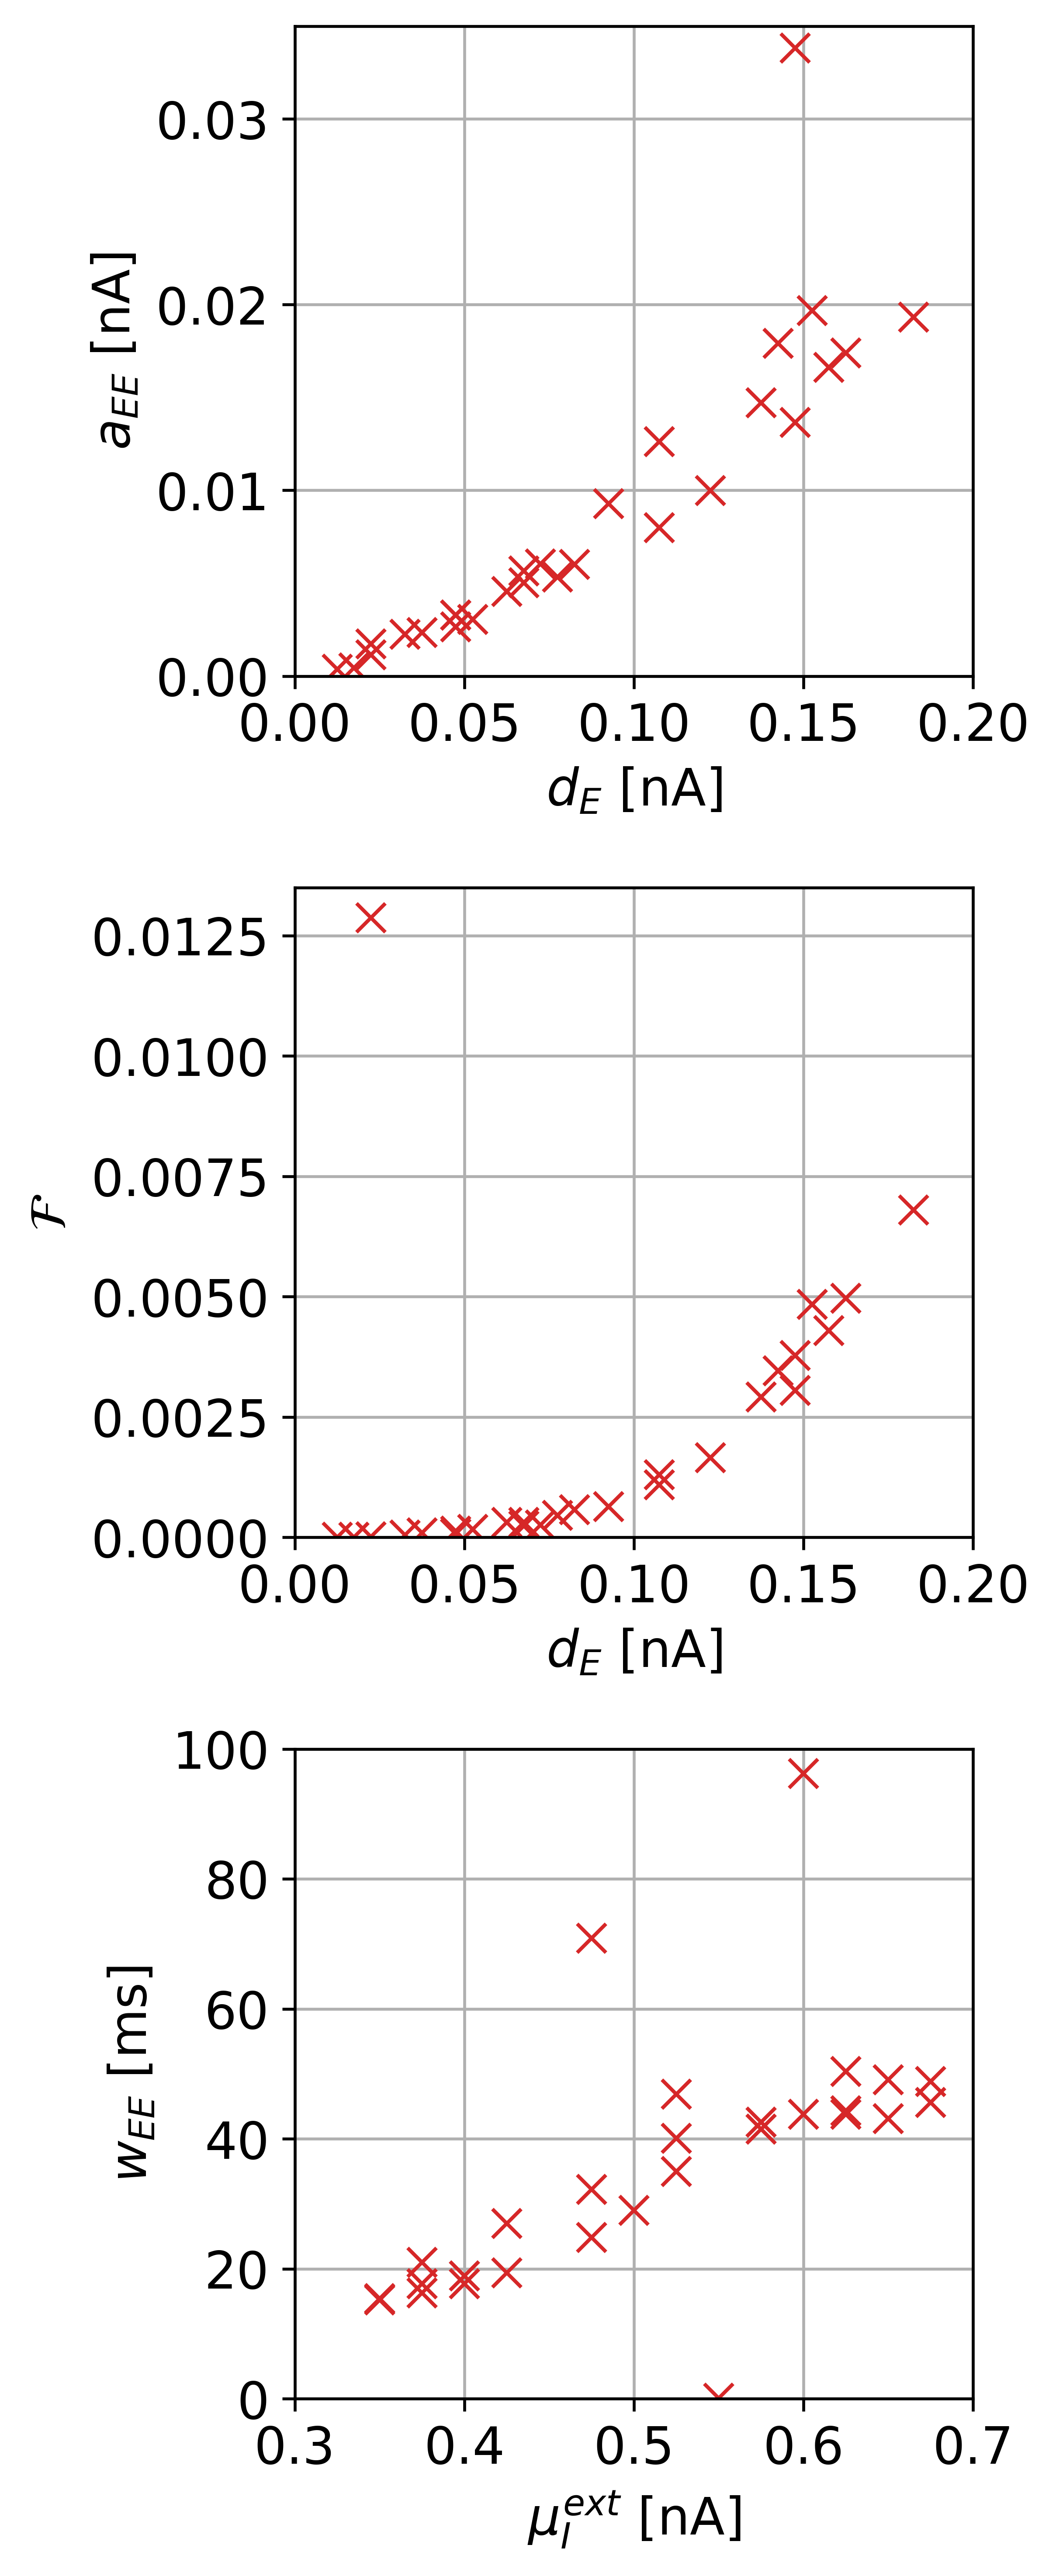
\includegraphics[width=\textwidth]{../rate_2.png}
\end{minipage}

\subsection{Up $\rightarrow$ down, $L_1$ cost}

\begin{minipage}{0.55\textwidth}
	\begin{itemize}
		\item inhibitory input to excitatory population for low external input to excitatory population, else no success
		\item no linear correlation of amplitude, cost, or width with one single parameter
		\item not successful for $\mu_E^\text{ext} = 0.425$ nA $\rightarrow$ why not?
	\end{itemize}
\end{minipage}
\begin{minipage}{0.43\textwidth}
	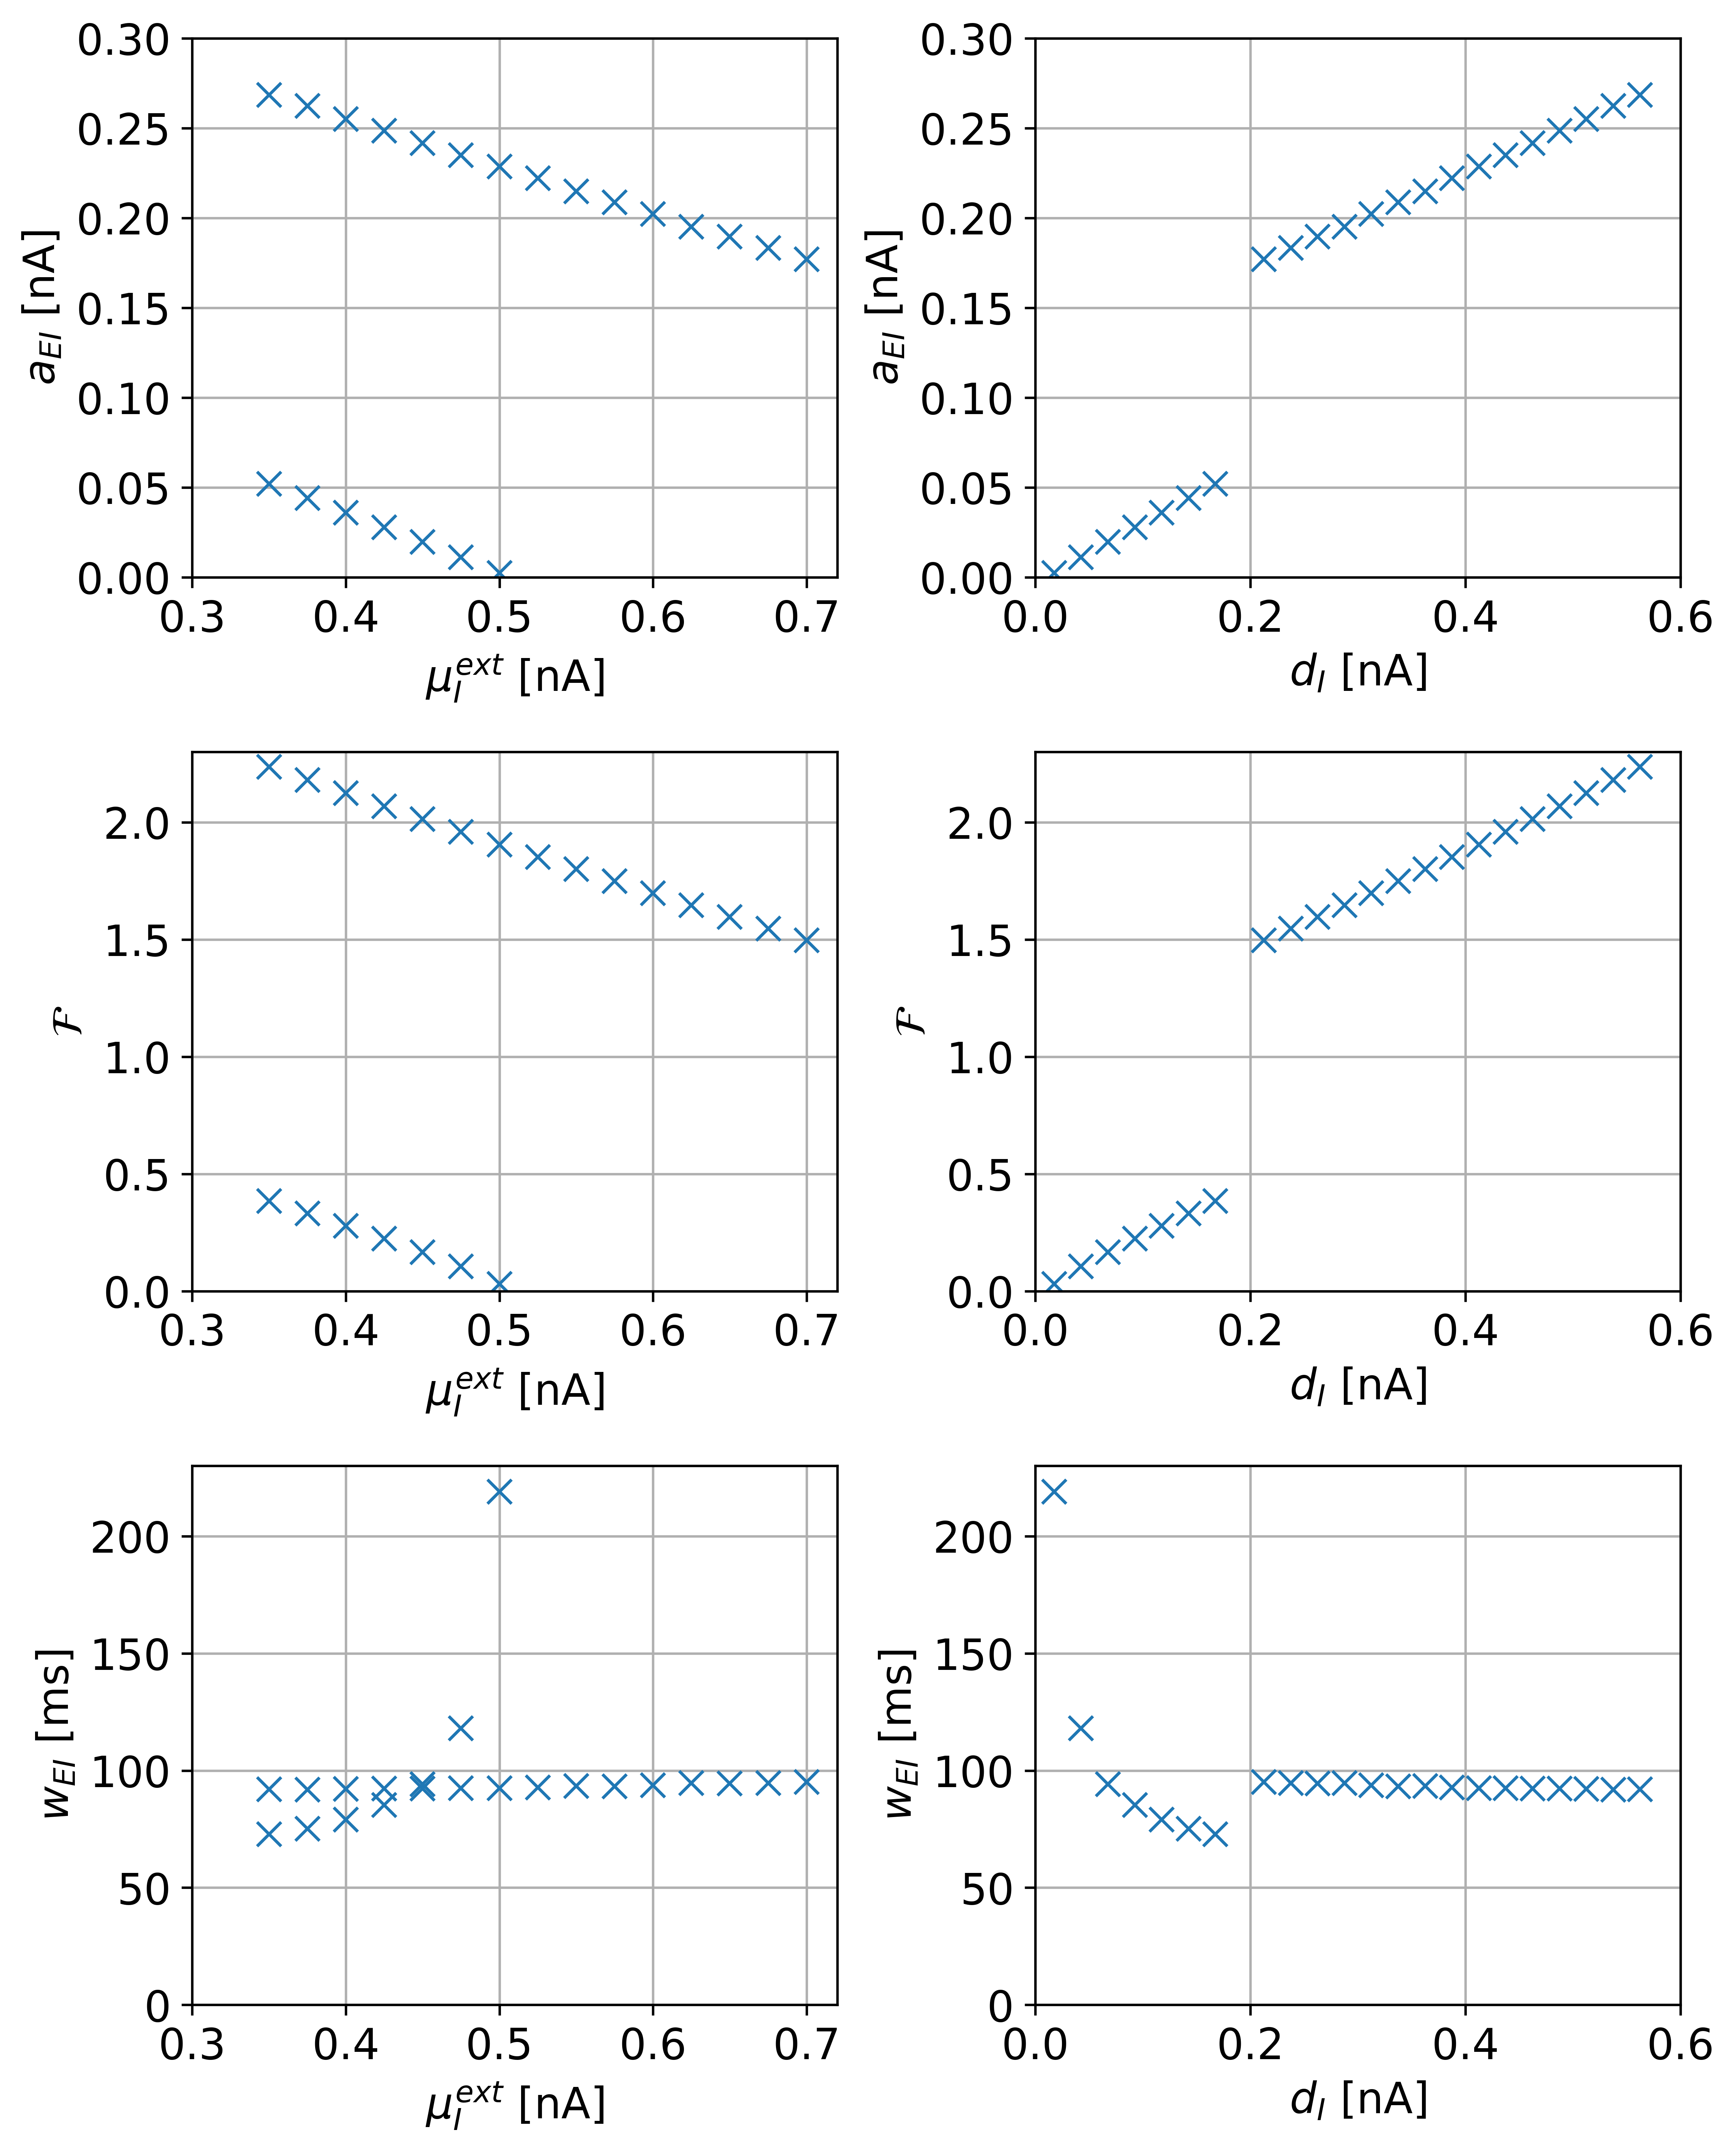
\includegraphics[width=\textwidth]{../rate_3.png}
\end{minipage}

\subsection{Up $\rightarrow$ down, $L_2$ cost}

\begin{minipage}{0.55\textwidth}
	\begin{itemize}
		\item inhibitory input to excitatory population with significantly larger (factor 5) amplitude for low external input to excitatory population, else no success
		\item no linear correlation of amplitude, cost, or width with one single parameter
	\end{itemize}
\end{minipage}
\begin{minipage}{0.43\textwidth}
	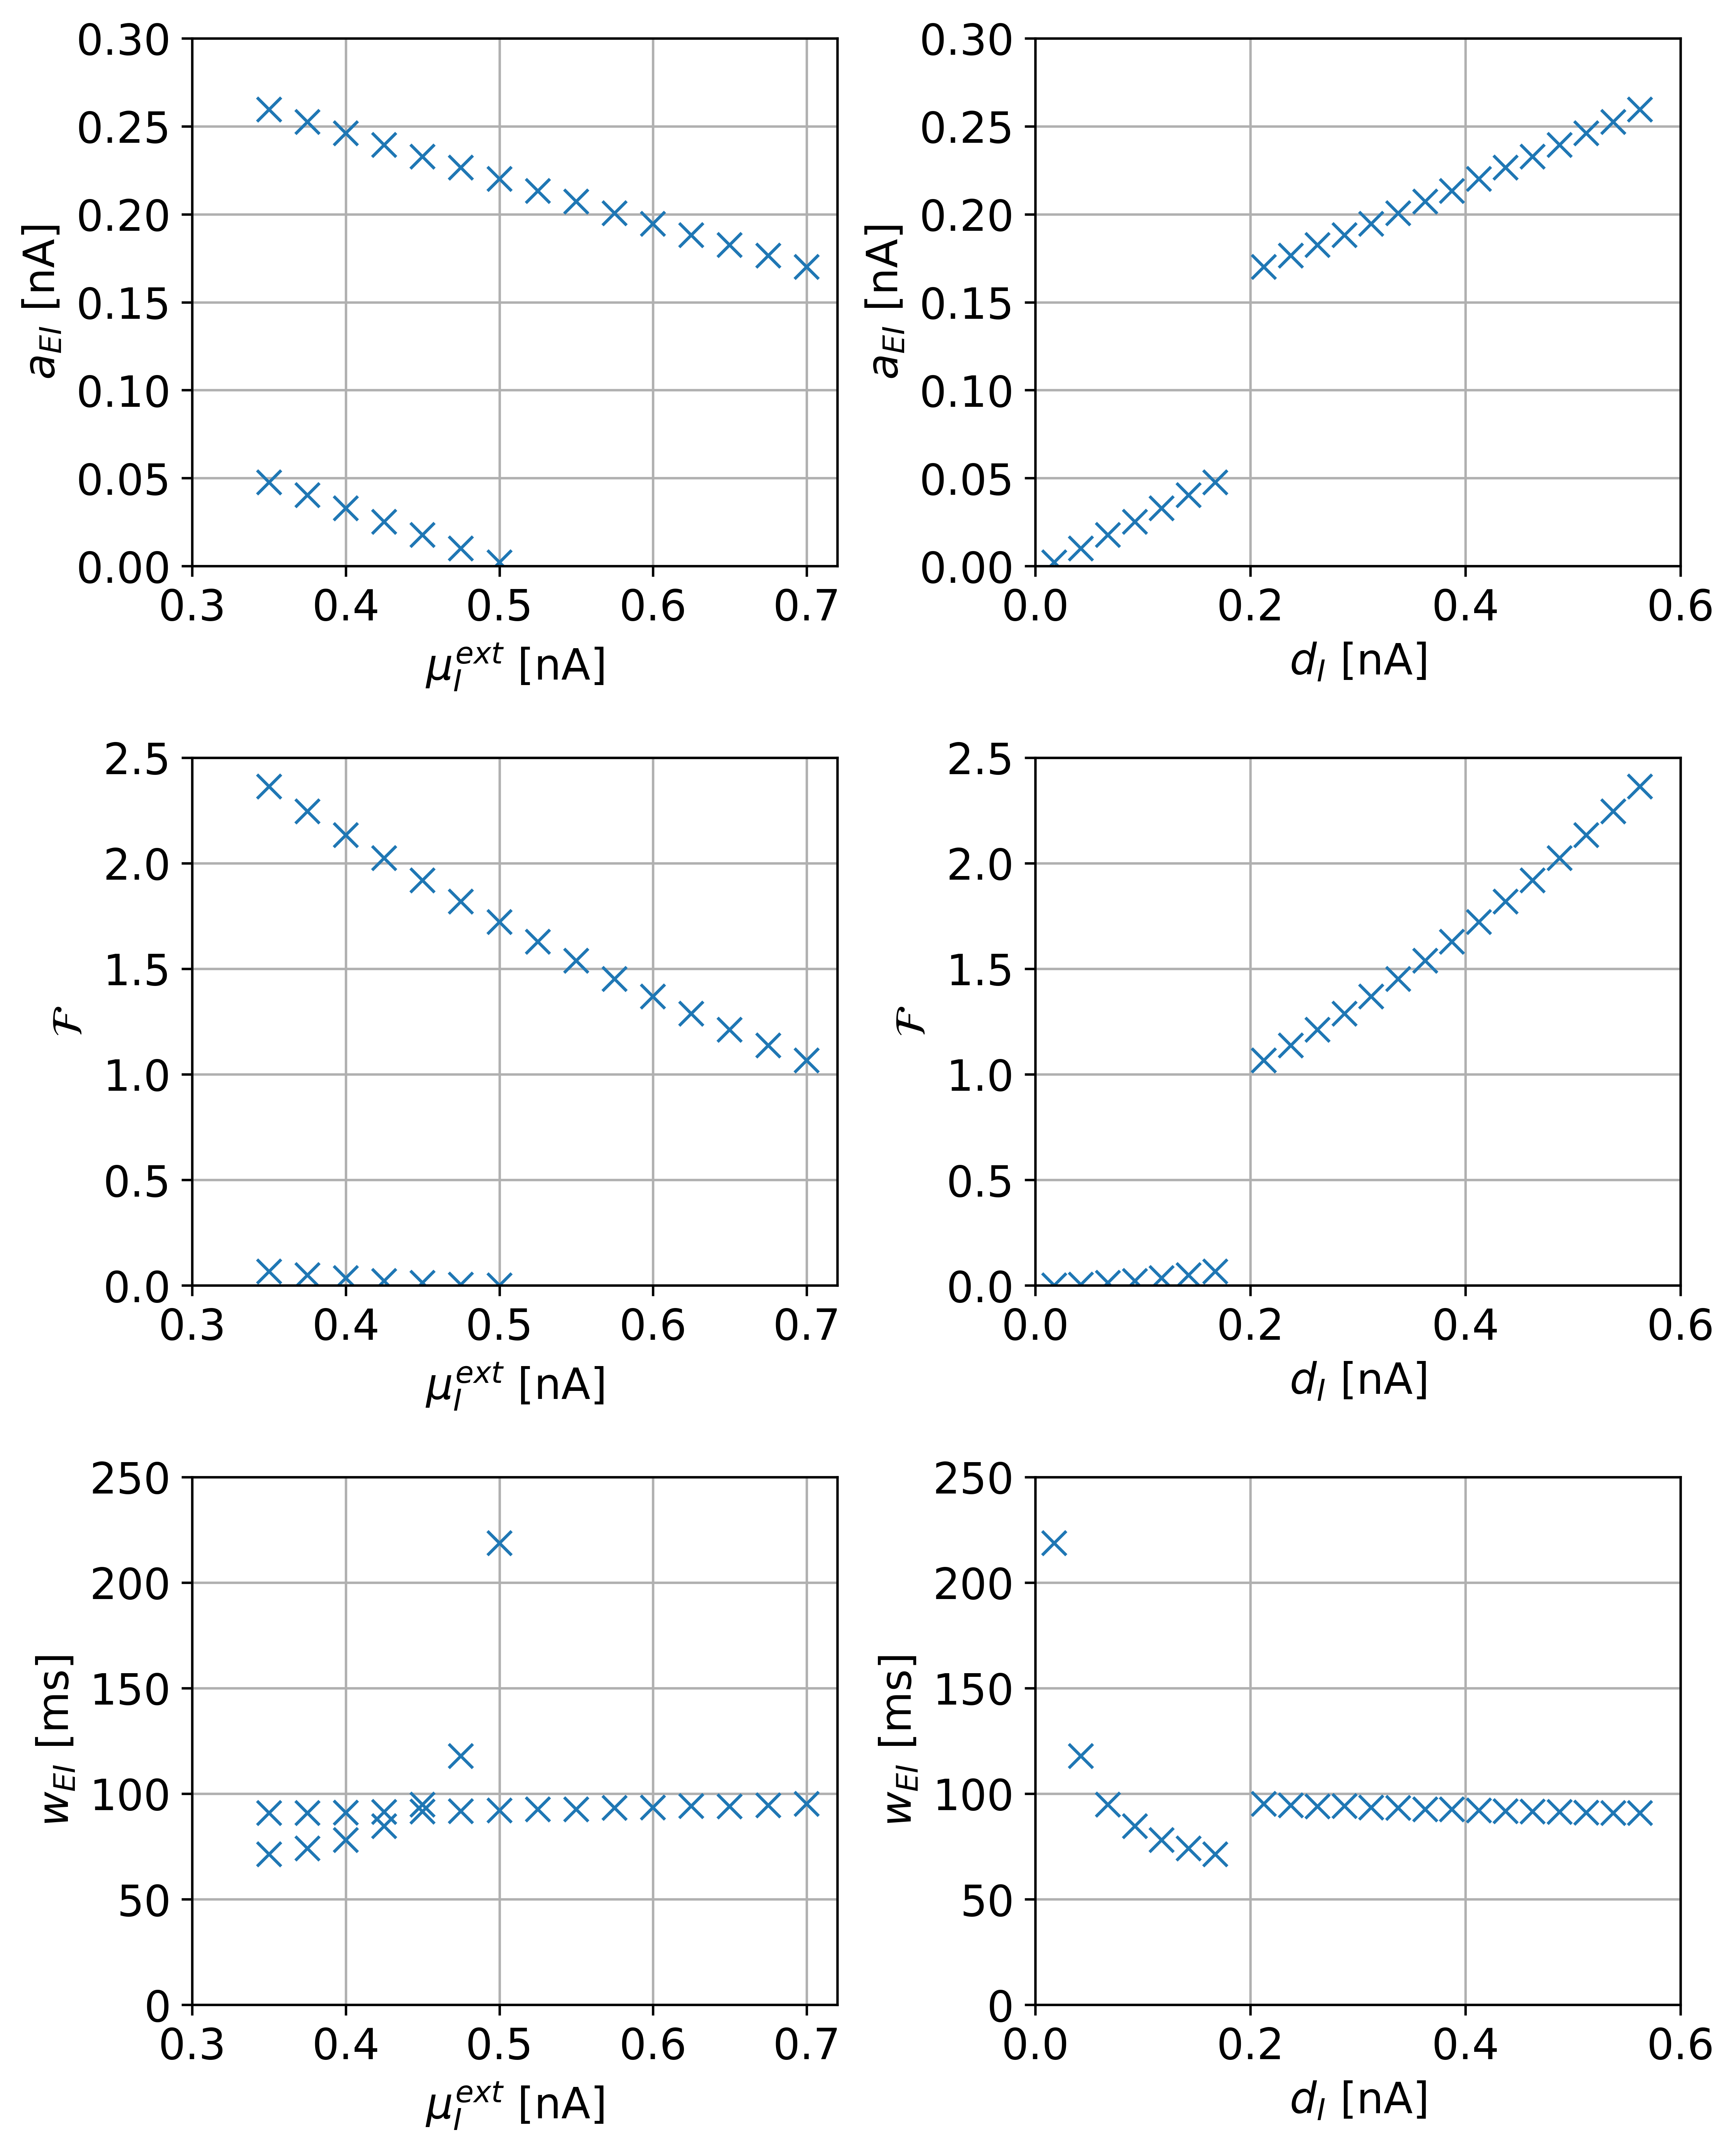
\includegraphics[width=\textwidth]{../rate_4.png}
\end{minipage}

\section{Optimal control with noise}

\begin{itemize}
	\item new variables $\mu_E^\text{OU}, \mu_I^\text{OU}$\\
	\begin{footnotesize}
		\begin{align*}
			\dot{\mu}_E - \frac{1}{\tau_E(t)} (J_{EE}\overline{s}_{EE}(t) + J_{EI} \overline{s}_{EI}(t) + \mu_E^\text{ext} - \mu_E(t) ) = 0 \hspace{5mm} \rightarrow \hspace{5mm} \dot{\mu}_E - \frac{1}{\tau_E(t)} (J_{EE}\overline{s}_{EE}(t) + J_{EI} \overline{s}_{EI}(t) + \mu_E^\text{OU} - \mu_E(t) ) = 0 \\ 
			\dot{\mu}_I - \frac{1}{\tau_I(t)} (J_{IE}\overline{s}_{IE}(t) + J_{II} \overline{s}_{II}(t) + \mu_I^\text{ext} - \mu_I(t) ) = 0 \hspace{5mm} \rightarrow \hspace{5mm} \dot{\mu}_I - \frac{1}{\tau_I(t)} (J_{IE}\overline{s}_{IE}(t) + J_{II} \overline{s}_{II}(t) + \mu_I^\text{OU} - \mu_I(t) ) = 0\\
			\dot{\mu}^\text{OU}_\alpha = \frac{\mu_\alpha^\text{ext} - \mu^\text{OU}}{\tau^\text{OU}} + \frac{\sigma^\text{OU} \xi(t)}{\sqrt{dt}}
		\end{align*}
	\end{footnotesize}
	\item noise leads to decrease in high-activity rates $r_{E}$ and $r_I$\\
	\includegraphics[width=0.5\textwidth]{../../current/gui/data_noise/HighRate_SigmaOU_1000.png}
	\includegraphics[width=0.5\textwidth]{../../current/gui/data_noise/HighRate_SigmaOU_10000.png}
	\item different ways to do averaging\\
	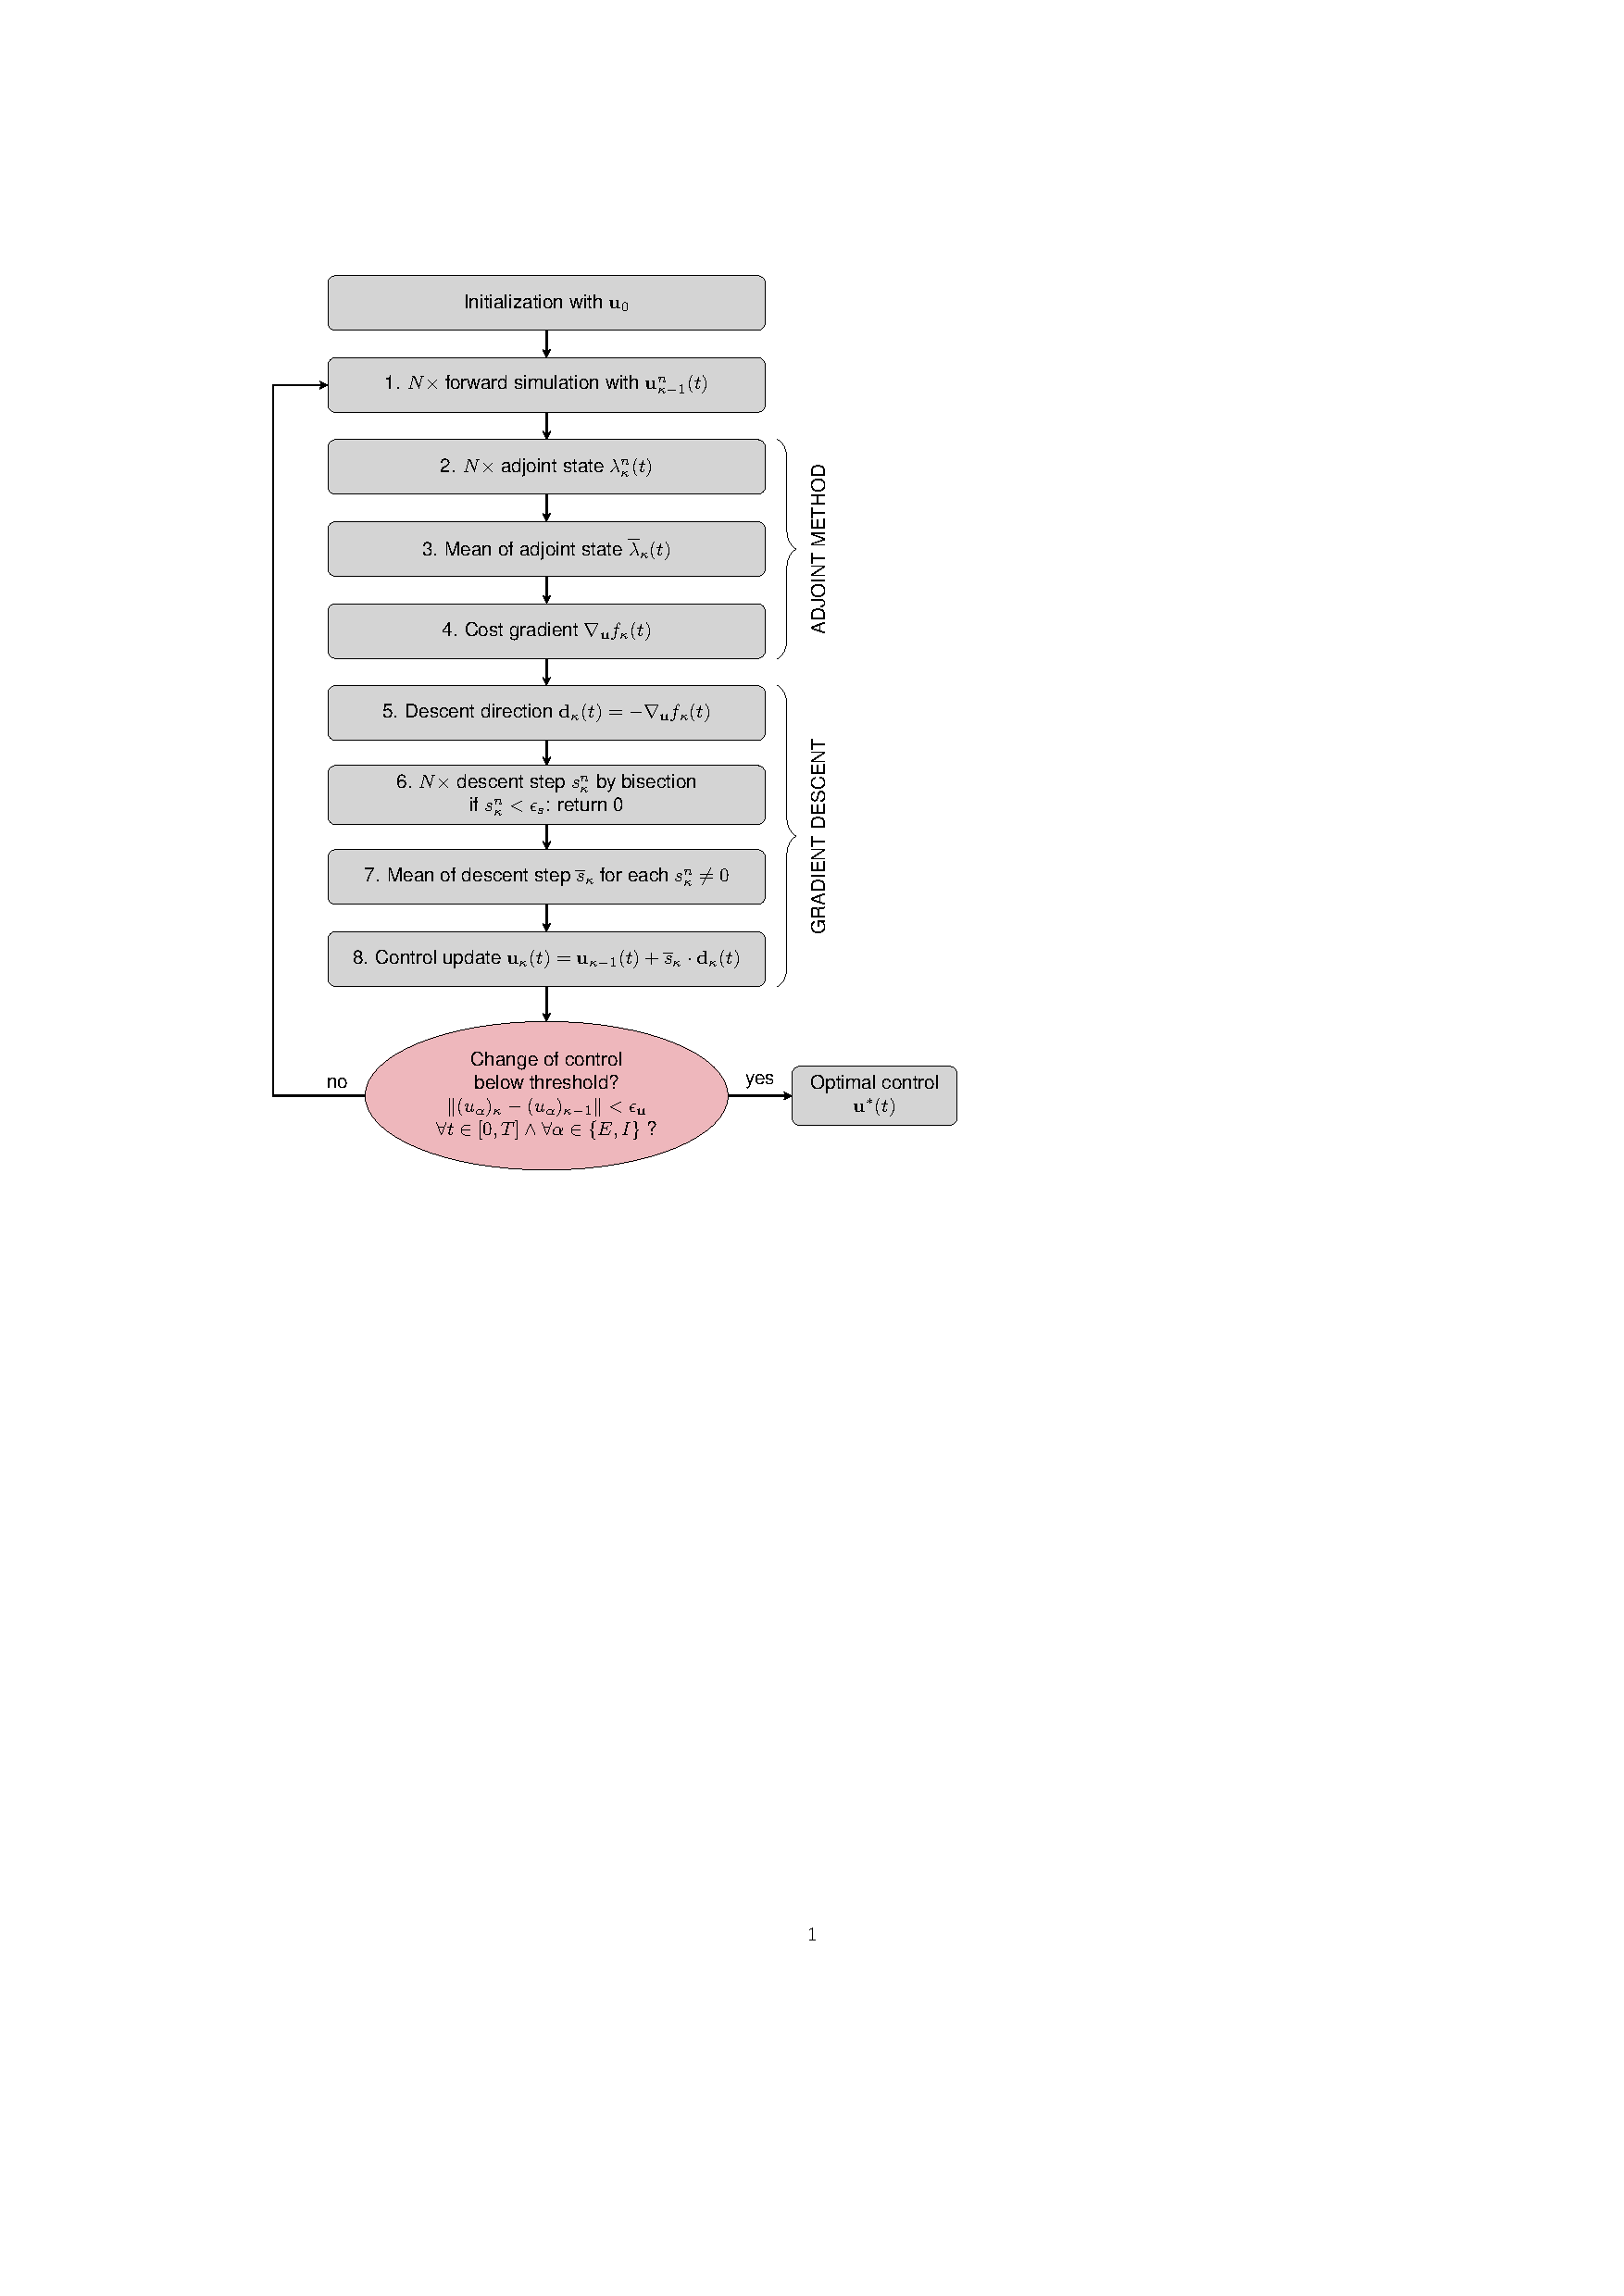
\includegraphics[width=0.5\textwidth, trim={5cm 18cm 12cm 5cm},clip]{./flowchart_noise.pdf}
	\item measure precision in $E$ and $I$ rate
	\item how to define \# noise realizations ($N$), \# iterations ($X$)/ abort criterion?
	\item overshooting is effective strategy that can be prevented by setting $W_{1,2} \gtrsim 1000$\\
	\includegraphics[width=0.5\textwidth]{../../current/gui/data_noise/3_.png}\\	
	\includegraphics[width=0.5\textwidth]{../../current/gui/data_noise/10_noise.png}
	\item use average of average costs up to $X$th iteration for abortion criterion\\
	$\overline{\mathcal{F}}^X = (\sum_{x=1}^{X} \sum_{n=1}^{N} \mathcal{F}_n^x) / (N \cdot X)$\\
	abort if $\overline{\mathcal{F}}^X < \overline{\mathcal{F}}^{X-1}$ and $\overline{\mathcal{F}}^X < \overline{\mathcal{F}}^{X-2}$ and $\overline{\mathcal{F}}^X > \overline{\mathcal{F}}^{X-3}$ and $\overline{\mathcal{F}}^X > \overline{\mathcal{F}}^{X-4}$ and $\overline{\mathcal{F}}^X > \overline{\mathcal{F}}^{X-5}$
	\item compute target rate from mean over $M$ realizations $\rightarrow N > M$ not reasonable
	\item $N$ depends on noise strength $\sigma^\text{OU}$?
	\item adding one more noise realization $N \rightarrow N+1$ should not change a lot
\end{itemize}


\end{document}
